\documentclass[11pt]{article}

\usepackage[letterpaper,margin=0.82in]{geometry}
\usepackage[T1]{fontenc}
\usepackage{lmodern}
\usepackage{microtype}
\usepackage{xcolor}
\usepackage{xspace}
\usepackage{enumitem}
\usepackage{amsmath}
\usepackage{booktabs}
\usepackage{tabularx}
\usepackage[most]{tcolorbox}
\usepackage[hidelinks]{hyperref}

\definecolor{commentgray}{RGB}{238,238,238}
\definecolor{responseblue}{RGB}{0,76,153}
\newcommand{\sysname}{COSMOS\xspace}
\newcommand{\response}[1]{\par\medskip\noindent\textbf{Response #1:}\ }
\newcommand{\changed}[1]{\textcolor{responseblue}{#1}}
\newenvironment{revisionquote}{\begin{quote}\itshape}{\end{quote}}
% Most evidence figures are single-column figures in the manuscript.  Display
% them at approximately their original physical width so that plot labels match
% the response-letter body text instead of being enlarged to page width.
\newcommand{\evidencefigure}[3][0.55\linewidth]{%
  \begin{center}
    \includegraphics[width=#1]{#2}\par
    \vspace{2pt}\small\textbf{#3}
  \end{center}}
\newtcolorbox{reviewcomment}{
  breakable,
  colback=commentgray,
  colframe=commentgray,
  boxrule=0pt,
  arc=0pt,
  left=7pt,right=7pt,top=7pt,bottom=7pt,
  before skip=8pt,after skip=5pt
}
\setlist{leftmargin=*,itemsep=3pt,topsep=4pt}
\setlength{\parindent}{0pt}
\setlength{\parskip}{5pt}

\begin{document}

\begin{center}
  {\Large\bfseries Response Letter for Manuscript TNET-2026-00030}\par
\end{center}

\vspace{12pt}
Dear EiC, AE, and Reviewers:

Thank you very much for your effort in reviewing our manuscript and for your valuable feedback. We have carefully addressed every point raised by the reviewers and revised the manuscript accordingly. In particular, we have made the following changes:

\begin{enumerate}[label=\arabic*.]
  \item Regarding the fixed CPU--memory demand-ratio assumption, we added CPU--memory demand-ratio measurements for open-source benchmarks in the Background and added an explanation of the model scope and boundary cases in the Discussion, as suggested by Reviewers 1, 2, and 3.
  \item We added analyses of node-level resource contention behavior in the Evaluation, including eviction frequency, eviction pressure caused by in-place scale-up, and the resulting impact on instance lifetime, as suggested by Reviewer 1.
  \item We added performance analyses under bursty workloads and high offered loads in the Evaluation, as suggested by Reviewers 1 and 2.
  \item We clarified the relationship between beneficial swaps and function relocation, and reported the function-relocation ratio and its actual performance impact during routing-plan updates in the Evaluation, as suggested by Reviewer 1.
  \item We added a discussion in Related Work to clarify the differences between \sysname and Golgi, as suggested by Reviewer 2.
  \item We revised the Introduction to clarify the novelty of \sysname, as suggested by Reviewer 2.
  \item We provided an effectiveness analysis for the components of \sysname in the Evaluation, as suggested by Reviewer 2.
  \item We evaluated the routing-plan generation overhead of \sysname using open-source invocation traces, as suggested by Reviewer 2.
  \item We added performance comparisons with the new Golgi baseline in the Evaluation, as suggested by Reviewer 2.
  \item We added an analysis comparing monotonic scale-up with size-specific prewarmed pools in the Discussion, as suggested by Reviewer 3.
  \item We revised the discussion of function request-demand prediction in the Discussion, as suggested by Reviewer 3, and added robustness experiments for function-load prediction accuracy in the Evaluation.
  \item We showed the impact of the scale-up mechanism on inter-function contention and eviction pressure in the Evaluation, as suggested by Reviewer 3.
  \item We reviewed and improved the overall writing, corrected the reported typographical errors, and moved selected material to the supplementary document to satisfy the manuscript page limit.
\end{enumerate}

Following this summary, we provide detailed responses to the comments raised by the three reviewers. For ease of review, we place each comment in a gray box and provide the corresponding response below it. Section, figure, and table references in this letter refer to the revised manuscript unless explicitly stated otherwise.

To help reviewers quickly locate the revised content, we attach the complete revised paper at the end of this PDF and highlight the modified parts in {\color{blue}BLUE}. We also upload the highlighted revised version in the “Supplementary Material for Review”.

We highly appreciate your time and effort in reassessing our manuscript.

Best regards,\\
Yunshan Jia, Junyi Shu, Chiheng Lou, Fangyue Liu, Chenbo Bi, and Xin Jin

\clearpage
\section*{Detailed Response to Reviewer 1}

\begin{reviewcomment}
\textbf{Comment 1.1:} On page 1, line 50, the authors say that ``54\% of functions exhibit substantial variation in resource usage under different inputs.'' However, on page 5, line 41, the authors claim that ``we assume this ratio remains invariant across requests of the same function.'' If the resource usage varies across different inputs for the same function, is it really reasonable to set this ratio using a static value for each function? In most cases, will the CPU-to-memory ratio remain fixed if the input changes? Will there be some cases in which the function could switch between compute-intensive and memory-intensive if the input is different? For example, when using a transformer model to do an inference task, the function could be compute-intensive with a long input sequence in the prefill stage, or memory-intensive when the output sequence in the decoding stage is very long. I suggest the authors add a detailed clarification to justify this fixed ratio assumption.
\end{reviewcomment}
\response{1.1} Thank you for your comment. The fixed CPU-to-memory demand-ratio assumption is motivated by the function decomposition that is central to serverless computing. A complex, stateful application is commonly decomposed into many fine-grained, dedicated, and independently scalable functions. These functions are typically stateless at the compute layer, with application state externalized to storage services. Because each function performs a well-defined task, different inputs often change the magnitude of its resource demand without changing its basic resource-use pattern.

We added empirical evidence in Section~II-B to validate this behavior. We use peak memory as the memory-demand metric because it determines the resource allocation required by a function instance:

\evidencefigure{figures/fig_ratio_stability_grid.pdf}{Revised Figure 2: CPU and memory usage across request inputs for serverless functions.}

\begin{revisionquote}
``Figure~2 further examines how CPU and memory usage co-vary as request inputs change. We randomly select ten functions from the open-source SeBS serverless benchmarking suite~[37], covering Web, multimedia, utility, machine-learning, and scientific workloads; their full names and characteristics are listed in Table~I. For each input, we measure the CPU time consumed and peak memory usage during task execution, averaged across repeated runs. Each point represents one input, and the red line is a per-function linear fit. The reported $R^2$ measures the goodness of fit, while CV is the coefficient of variation of the per-input CPU-to-peak-memory ratios. The figure omits graph-mst due to space because it closely matches graph-bfs ($R^2=0.996$, CV=27.9\%).

Eight of the ten benchmarks exhibit strong input-dependent CPU--memory coupling: their CPU and memory demands increase along a stable function-specific direction, with linear-fit $R^2$ values between 0.974 and 0.999 and ratio CVs from 5.2\% to 29.7\%. Thus, although inputs change demand magnitude, the relative CPU-to-peak-memory profile remains broadly stable and does not typically switch between compute- and memory-intensive behavior.''
\end{revisionquote}

\begin{quote}\small
[37] M.~Copik, G.~Kwasniewski, M.~Besta, M.~Podstawski, and T.~Hoefler, ``SeBS: A serverless benchmark suite for function-as-a-service computing,'' in \emph{Proceedings of the 22nd International Middleware Conference}, ser. Middleware '21, p. 64--78.
\end{quote}

The transformer example raised by the reviewer further illustrates why function boundaries matter. Prefill--decode disaggregation has become a mainstream design in modern LLM serving systems, as exemplified by DistServe (OSDI~'24). In this design, the prefill and decoding stages are deployed as separate, independently scalable components. If these stages are represented as separate serverless functions, the prefill function and decoding function each have a relatively consistent resource profile, even though the complete inference application contains both compute-intensive and memory-intensive stages. Accordingly, we clarified the rationale, applicability, and boundary of the resource-profile model in Section~VII:

\begin{revisionquote}
``Serverless computing commonly decomposes complex, stateful applications into fine-grained, dedicated, stateless functions that scale independently, with state externalized to storage services. Because each function performs a well-defined task, request inputs often change demand magnitude rather than its qualitative CPU-to-memory profile, as illustrated by eight of the ten functions in Figure~2. Motivated by this structure, COSMOS models each function with a stable CPU-to-memory demand ratio and a variable demand magnitude.

Single-resource-dominant functions, such as video-processing and uploader in Figure~2, can still be represented by a conservative fixed resource ratio. This may over-allocate the less-variable resource but preserves normal system operation. Specialized support would require extending the demand model and SwapCapacity routine to allow the ratio to vary with request size.

The current model does not directly support a complex function whose resource profile changes qualitatively across requests. Such a function could be divided into virtual functions by request type or refactored into dedicated stages, each with a stable profile. We leave direct support for such functions to future work.''
\end{revisionquote}

\begin{quote}\small
Y.~Zhong, S.~Liu, J.~Chen, J.~Hu, Y.~Zhu, X.~Liu, X.~Jin, and H.~Zhang, ``DistServe: Disaggregating prefill and decoding for goodput-optimized large language model serving,'' in \emph{18th USENIX Symposium on Operating Systems Design and Implementation (OSDI 24)}, 2024, pp. 193--210.
\end{quote}

\begin{reviewcomment}
\textbf{Comment 1.2:} I still have concerns about the resource contention issue. The paper also acknowledges that dynamic resizing and eviction can cause resource contention and eviction amplification on a node. The authors try to mitigate this by using complementary swarming and routing requests with similar demand to the same node. However, the evaluation mainly reports end-to-end utilization and latency improvements. It does not provide a detailed analysis of node-level contention behavior, such as eviction frequency, eviction cascades, or worst-case interference when workloads spike. If possible, is there any theoretical bound or backoff method on such contention impact? Without such analysis, it is hard to validate how the system behaves under extreme cases.
\end{reviewcomment}
\response{1.2} Thank you for your comment. Because \sysname relies on heuristic online routing and scheduling whose decisions depend on the workload composition, available node slack, and timing of load changes, deriving a precise workload-independent theoretical bound on the impact of contention is difficult. Nevertheless, we can qualitatively characterize the worst-case behavior.

Suppose that a function experiences a sudden load increase that exceeds the available slack and processing capacity of every server to which that function is routed before the next routing-plan update. In this worst case, all of these servers can become saturated: requests of the bursty function may accumulate, its scale-up requests may trigger pod evictions, and the co-located functions on these servers may also experience resource contention, additional cold starts, and increased latency. Complementary swarming confines this impact to the function's assigned server set unless that function itself is distributed across the entire cluster, but it cannot completely prevent interference within that set under this extreme condition.

However, this synchronized worst case is empirically difficult to reach because a burst must exhaust the available capacity of all servers assigned to the function at the same time. For a short-term burst, available node slack and warm instances can absorb part of the transient increase, allowing \sysname to process the burst and recover faster than the baselines. If the load change persists, it is incorporated into the next routing-plan update, which repartitions function demand to rebalance resource allocation against the new workload. To examine whether the above worst-case risk materializes in practice, we added experiments in Section~VI-C that measure behavior under a workload spike, eviction frequency, eviction pressure caused by in-place scale-up, and the resulting impact on instance lifetime. We also added high-load measurements to evaluate \sysname under extreme offered-load conditions:

First, we measure minute-level cold-start rate and 99th-percentile tail latency during a representative burst. The results show that COSMOS incurs fewer cold starts, has a smaller latency spike, and recovers faster than the baselines:

\evidencefigure[0.5\linewidth]{figures/fig_temporal_coldstart_latency.pdf}{Revised Figure 11: Minute-level cold-start rate and 99th-percentile tail latency under bursty load and routing-plan updates.}

\begin{revisionquote}
``Figure~11 shows the minute-level cold-start rate and 99th-percentile tail latency after excluding the first five minutes of system warm-up. \ldots{} Between minutes 26 and 28, the invocation rate of \textbf{graph-pagerank} rises by about $5\times$. This burst is particularly challenging because \textbf{graph-pagerank} is among the most resource-demanding benchmarks. As shown in the figure, the burst
causes sharp increases in both cold starts and tail latency for all systems. Nevertheless, COSMOS incurs fewer cold starts and a smaller latency spike than the baselines, and its tail latency quickly returns toward its pre-burst level. In contrast, the baselines retain elevated tail latency and recover more slowly.''
\end{revisionquote}

Second, we quantify the pod-eviction frequency observed during the same burst experiment. COSMOS has the lowest pod-eviction rate among all evaluated systems:

\begin{revisionquote}
``Moreover, COSMOS incurs fewer cold starts than the baselines, and its pod-eviction rate is 1.433 events/min, 60.6\% lower than the best baseline in Table~II. These results show that routing-plan relocation does not increase observable instance churn.''
\end{revisionquote}

\begin{center}
\small
\begin{tabular}{lccccc}
\toprule
\textbf{System} & \textbf{Palette} & \textbf{FaaSCache} & \textbf{Golgi} & \textbf{Golgi-NoCC} & \textbf{COSMOS} \\
\midrule
Average rate (events/min) & 5.433 & 4.500 & 8.967 & 3.633 & \textbf{1.433} \\
\bottomrule
\end{tabular}\par
\vspace{2pt}\small\textbf{Revised Table II: Pod eviction rate among COSMOS and baselines for Figure~11.}
\end{center}

Third, we measure how often in-place scale-up is absorbed by available node slack rather than translated into eviction pressure. Most scale-up events of \sysname do not cause eviction:

\begin{revisionquote}
``Figure~13 reports the fraction of scale-up events that trigger pod eviction across offered loads, \ldots{} Together with the overall pod-eviction rate and cold-start results, these metrics evaluate whether the eviction-amplification risk of in-place scaling translates into increased instance churn. For \sysname, the fraction of scale-ups causing eviction first increases and then
decreases with load. At light loads, eviction events initially grow faster than
scale-up events. As load increases further, however, scale-ups become much more
frequent and are predominantly absorbed by available node resources. From 45\%
to 100\% load, the number of scale-up events increases by $6.34\times$, whereas
the number causing eviction increases by only $1.48\times$; consequently, their
fraction falls from 5.05\% to 1.18\%.
Across \sysname and all baselines, fewer than 15\% of scale-up events cause an
eviction, indicating that in-place scale-up usually preserves warm instances
rather than triggering additional cold starts.''
\end{revisionquote}

\evidencefigure[0.47\linewidth]{figures/fig_scaleup_absorption.pdf}{Revised Figure 13: Fraction of scale-up events that cause pod eviction.}

Fourth, we examine instance lifetime to evaluate the cumulative impact of eviction and churn. The results show that COSMOS shifts instance lifetimes toward longer durations:

\evidencefigure{figures/fig_instance_lifetime_cdf.pdf}{Revised Figure 14: Instance-lifetime distributions.}

\begin{revisionquote}
``Figure~14 compares the instance-lifetime distributions
of four representative functions. \ldots{} Consistent with this result, the instance-lifetime CDFs in Figure~14 shift toward longer lifetimes under COSMOS. We observe the same trend for the remaining six functions. These results show that monotonic scale-up does not increase instance churn.''
\end{revisionquote}

We evaluate instance lifetime because it captures the aggregate operational impact of eviction and churn more directly than a recursive request-level eviction cascade. A request-level cascade would require tracing a causal lineage from an evicted pod to its reconstruction and then to subsequent evictions. However, in serverless systems, a pod is shared by multiple invocations, and an evicted pod has no one-to-one correspondence with a subsequently created pod of the same function. Thus, the execution model does not define a unique reconstruction chain. At the function level, correlated eviction peaks may be observed, but they do not identify a unique recursive cascade. We therefore evaluate directly observable eviction pressure and impacts, and show that COSMOS achieves low observable instance churn under the evaluated workloads and configuration.

Finally, we report the high-load performance testing results to reflect the system performance under extreme loads:

\begin{revisionquote}
``We generate user traffic based on the Azure Functions Dataset~[15]. \ldots{} Offered-load levels are created by proportionally scaling all traces, preserving their temporal patterns across traffic levels. Load is reported as a percentage of cluster CPU capacity, where 100\% denotes aggregate profiled CPU demand matching the cluster's allocatable CPU capacity.''
\end{revisionquote}

\begin{quote}\small
[15] M.~Shahrad, R.~Fonseca, I.~Goiri, G.~Chaudhry, P.~Batum, J.~Cooke, E.~Laureano, C.~Tresness, M.~Russinovich, and R.~Bianchini, ``Serverless in the wild: Characterizing and optimizing the serverless workload at a large cloud provider,'' in \emph{Proceedings of the 2020 USENIX Annual Technical Conference}, California, USA, 2020, pp. 205--218.
\end{quote}

\begin{center}

\includegraphics[width=0.60\linewidth]{figures/fig_main_legend.pdf}\\[-6pt]
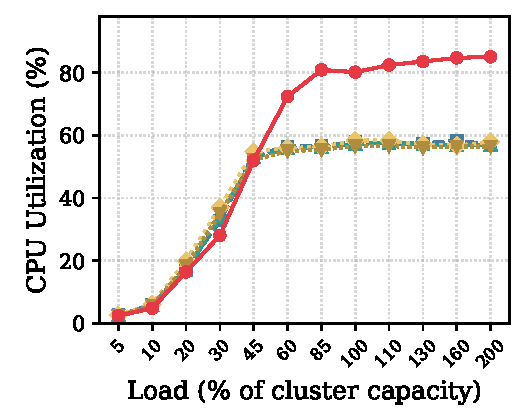
\includegraphics[width=0.31\linewidth]{figures/fig_main_cpu.pdf}\hfill
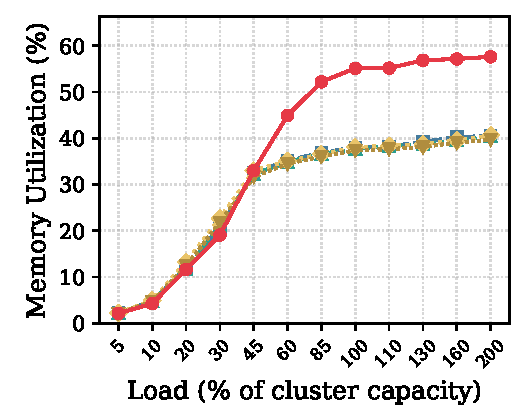
\includegraphics[width=0.31\linewidth]{figures/fig_main_mem.pdf}\hfill
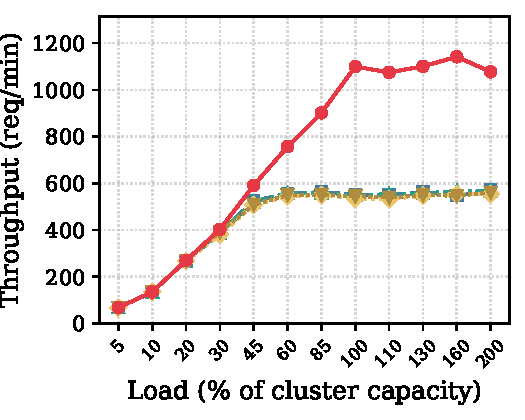
\includegraphics[width=0.31\linewidth]{figures/fig_main_throughput.pdf}\par
\small\textbf{Revised Figure 7: Main-experiment comparison across offered loads: (a) CPU utilization, (b) memory utilization, and (c) task throughput.}
\end{center}

\vspace{-20pt}

\evidencefigure[0.40\linewidth]{figures/fig_main_latency.pdf}{Revised Figure 8: 99th-percentile latency across offered loads.}

\begin{revisionquote}
``
Figures~7 and~8 compare \sysname with the baselines across offered loads from 5\% to 200\% of cluster capacity. Unless otherwise stated, all reported differences are relative to the best-performing baseline for the corresponding metric at each load. At light loads (5\%--30\%), all systems achieve nearly identical throughput, with differences within 5.82\%, because resources are abundant and scheduling efficiency is not yet a bottleneck. The baselines also perform similarly, except that Golgi generally incurs higher tail latency, suggesting that its relatively aggressive overcommitment involves a tail-latency trade-off.

The advantage of \sysname emerges as the offered load approaches cluster capacity. At 45\% load, \sysname improves throughput by 12.83\% and reduces the 99th-percentile latency by 78.77\%. From 60\% to 200\% load, all baselines reach a similar throughput ceiling. In contrast, \sysname improves CPU utilization by 28.34\%--46.91\%, memory utilization by 27.76\%--45.00\%, and throughput by 35.63\%--101.31\%. Over the same range, \sysname reduces the 99th-percentile latency by 8.19\%--28.94\%, showing that its throughput gains do not compromise tail latency.

These gains stem from two complementary mechanisms. Complementary swarming narrows each node's function set to improve reuse while matching resource profiles to node capacity to reduce fragmentation. Monotonic scale-up further reduces over-provisioning and cold starts, sustaining higher utilization and throughput as load rises.''
\end{revisionquote}

Taken together, these measurements show that, although the qualitative worst case described above cannot be completely excluded, it does not materialize under the evaluated bursty and high-load workloads. \sysname maintains a low eviction frequency, mitigates burst-induced latency spikes, preserves longer-lived warm instances, and sustains its performance advantage under high-load conditions.

\begin{reviewcomment}
\textbf{Comment 1.3:} The overhead and side effects of beneficial swaps are not clearly analyzed. The routing algorithm allows beneficial swaps, which may evict already placed workloads to improve resource utilization. While the paper reports the overall routing-plan generation overhead and claims it is small, it does not analyze how often these swaps happen in practice or how much overhead they introduce. For example, swaps could disturb warm placements or trigger additional rescheduling overhead. A more detailed evaluation of swap frequency and its impact on system stability would strengthen the paper.
\end{reviewcomment}
\response{1.3} Thank you for your suggestion. We added an analysis in Section~VI-C to quantify both the overall demand relocation caused by routing-plan updates and their observable runtime impact, including cold starts, tail latency, and pod-eviction rate.

We evaluate plan-level demand relocation rather than the raw count of individual beneficial swaps because the manuscript defines this metric as the aggregate effect of internal swap operations on the deployed routing plan. We therefore use the runtime-visible aggregate relocation as the experimental metric:

\begin{revisionquote}
``Figure~12 and Table~II further examine the routing-plan updates in the
experiment shown in Figure~11. The figure
decomposes the net per-function demand relocation between six pairs of
consecutive routing plans, while the table reports the observed runtime pod
eviction rates. This plan-level metric captures the aggregate effect of
beneficial swaps on function-load placement, rather than counting internal swap
operations, which are never deployed individually. The even-numbered updates relocate
only 40.4\%--51.7\% of total demand,
substantially less than the 72.0\%--76.9\% relocated by the odd-numbered updates,
demonstrating the effect of partial~updates.

The overall relocated share remains relatively high because \sysname deliberately
adopts an aggressive reallocation policy: upon detecting an increase in a
function's load, it reallocates that function's full demand rather than only the
increment. This design prioritizes concentrating each function on fewer servers,
as function concentration has a greater performance impact than minimizing the
magnitude of each load adjustment. Routing-plan changes are applied lazily as subsequent requests arrive rather than by eagerly migrating all affected instances, so the plan-level relocation overstates the workload immediately affected at runtime. ''
\end{revisionquote}

\evidencefigure[0.5\linewidth]{figures/fig_swap_analysis.pdf}{Revised Figure 12: Per-function demand relocation between consecutive COSMOS routing plans.}

The added results show that the relocation does not translate into additional observable instability:

\begin{revisionquote}
``As shown in Figure~11, \sysname does not exhibit routing-update-induced tail-latency spikes outside the burst window. Moreover, \sysname incurs fewer
cold starts than the baselines, and its pod-eviction rate is 1.433 events/min,
60.6\% lower than the best baseline in Table~II. These
results show that routing-plan relocation does not increase observable instance
churn.''
\end{revisionquote}

\evidencefigure{figures/fig_temporal_coldstart_latency.pdf}{Revised Figure 11: Minute-level cold-start rate and 99th-percentile tail latency under bursty load and routing-plan updates.}

\begin{center}
\small
\begin{tabular}{lccccc}
\toprule
\textbf{System} & \textbf{Palette} & \textbf{FaaSCache} & \textbf{Golgi} & \textbf{Golgi-NoCC} & \textbf{COSMOS} \\
\midrule
Average rate (events/min) & 5.433 & 4.500 & 8.967 & 3.633 & \textbf{1.433} \\
\bottomrule
\end{tabular}\par
\vspace{2pt}\small\textbf{Revised Table II: Pod eviction rate among COSMOS and baselines for Figure~11.}
\end{center}

\begin{reviewcomment}
\textbf{Comment 1.4:} Some minor typo issues:

Fig. 10, ``Comsupmtion'' $\rightarrow$ ``Consumption''

Fig. 6, ``acale-up'' $\rightarrow$ ``scale-up''

On page 4, line 22, ``a increment-only strategy'' $\rightarrow$ ``an increment-only strategy''
\end{reviewcomment}
\response{1.4} Thank you for pointing out these issues. We have carefully checked the manuscript and figures, corrected all three issues identified by the reviewer, and also reviewed the manuscript for other similar typographical errors.

\section*{Detailed Response to Reviewer 2}

\begin{reviewcomment}
\textbf{Comment 2.1:} This paper assumes that the CPU-to-memory ratio remains invariant within the same function. However, in Section 2.1, the analysis of real-world functions only shows that resource demand varies across requests; it does not establish that the CPU-to-memory ratio is invariant for a function. So, I am concerned about whether this assumption is valid and, if not, how it may affect the design of COSMOS. Further, you state in the related work section that, unlike Golgi, COSMOS considers per-request resource demand variation. However, the current design appears to consider only variations in the magnitude of resource demand, rather than variations in the CPU-to-memory ratio itself. This makes the difference less clear.
\end{reviewcomment}
\response{2.1} Thank you for your comment. COSMOS currently assumes a fixed ratio of CPU-to-memory resource demand for each serverless function. We added empirical validation in Section~II-B to examine whether the CPU-to-memory ratio remains stable within the same function as request inputs change. The results show that most evaluated functions satisfy this modeling assumption: eight of the ten SeBS benchmarks exhibit a stable function-specific CPU-to-peak-memory profile, even though their demand magnitude changes across inputs:

\begin{revisionquote}
``Figure~2 further examines how CPU and memory usage co-vary as request inputs change. We randomly select ten functions from the open-source SeBS serverless benchmarking suite~[37], covering Web, multimedia, utility, machine-learning, and scientific workloads; their full names and characteristics are listed in Table~I. For each input, we measure the CPU time consumed and peak memory usage during task execution, averaged across repeated runs. Each point represents one input, and the red line is a per-function linear fit. The reported $R^2$ measures the goodness of fit, while CV is the coefficient of variation of the per-input CPU-to-peak-memory ratios. The figure omits graph-mst due to space because it closely matches graph-bfs ($R^2=0.996$, CV=27.9\%). Eight of the ten benchmarks exhibit strong input-dependent CPU--memory coupling: their CPU and memory demands increase along a stable function-specific direction, with linear-fit $R^2$ values between 0.974 and 0.999 and ratio CVs from 5.2\% to 29.7\%. Thus, although inputs change demand magnitude, the relative CPU-to-peak-memory profile remains broadly stable and does not typically switch between compute- and memory-intensive~behavior.''
\end{revisionquote}

\begin{quote}\small
[37] M.~Copik, G.~Kwasniewski, M.~Besta, M.~Podstawski, and T.~Hoefler, ``SeBS: A serverless benchmark suite for function-as-a-service computing,'' in \emph{Proceedings of the 22nd International Middleware Conference}, ser. Middleware '21, p. 64--78.
\end{quote}

\evidencefigure{figures/fig_ratio_stability_grid.pdf}{Revised Figure 2: CPU and memory usage across request inputs for serverless functions.}

We also revised the Discussion to explain why this assumption is consistent with the serverless function-decomposition model, how single-resource-dominant functions can be represented conservatively, and where the boundary of the current model lies:

\begin{revisionquote}
``Serverless computing commonly decomposes complex, stateful applications into fine-grained, dedicated, stateless functions that scale independently, with state externalized to storage services. Because each function performs a well-defined task, request inputs often change demand magnitude rather than its qualitative CPU-to-memory profile, as illustrated by eight of the ten functions in Figure~2. Motivated by this structure, COSMOS models each function with a stable CPU-to-memory demand ratio and a variable demand magnitude.

Single-resource-dominant functions, such as video-processing and uploader in Figure~2, can still be represented by a conservative fixed resource ratio. This may over-allocate the less-variable resource but preserves normal system operation. Specialized support would require extending the demand model and SwapCapacity routine to allow the ratio to vary with request size.

The current model does not directly support a complex function whose resource profile changes qualitatively across requests. Such a function could be divided into virtual functions by request type or refactored into dedicated stages, each with a stable profile. We leave direct support for such functions to future work.''
\end{revisionquote}

In addition, we revised the Related Work to clarify the distinction between COSMOS and Golgi:

\begin{revisionquote}
``In contrast, COSMOS models demand to coordinate resource allocation and function-load partitioning, mitigating fragmentation and burst-induced performance variation. Golgi~[43] maintains differently sized, overcommitted instances but routes requests solely by latency predictions and online performance statistics. This reactive design is sensitive to transient variations and forgoes resource-profile-aware instance reuse.''
\end{revisionquote}

\begin{quote}\small
[43] S.~Li, W.~Wang, J.~Yang, G.~Chen, and D.~Lu, ``Golgi: Performance-aware, resource-efficient function scheduling for serverless computing,'' in \emph{Proceedings of the 2023 ACM Symposium on Cloud Computing}, ser. SoCC '23, p. 32--47.
\end{quote}

\begin{reviewcomment}
\textbf{Comment 2.2:} It would be better to clarify the novelty. Each design components, i.e., request routing, resource-aware placement, and in-place vertical scaling--- do not appear entirely new in isolation. For example, in terms of request routing, I think it is almost similar to Golgi. It would be better to clear which part constitutes the real technical novelty, and which part is mainly an integration of existing ideas. I would encourage the authors to sharpen this distinction; otherwise, it will be difficult to know what the real contribution is. Further, the performance breakdown of COSMOS helps understand each components' performance gains.
\end{reviewcomment}
\response{2.2} Thank you for your suggestion. We agree that the individual mechanisms used by COSMOS, such as request routing, resource-aware placement, and vertical scaling, are not entirely new in isolation. The technical novelty of COSMOS lies in \textbf{proactively} modeling function-level and request-level resource-demand heterogeneity and using this model to jointly guide inter-node resource allocation and intra-node load partitioning.

This proactive approach is not a trivial change from making decisions reactively: it requires resource demand to be modeled reliably before a request executes and requires the resulting model to coordinate decisions at both the inter-node and intra-node levels. This modeling choice is inspired by the decomposition characteristic of serverless computing. Decomposing complex, stateful applications into fine-grained, dedicated, stateless functions offers an opportunity to characterize resource-use patterns and their input-dependent variation at the function level. Based on this observation, COSMOS models both cross-function resource diversity and within-function demand variation, then incorporates them into complementary swarming and monotonic scale-up scheduling. We clarified this point in Section~I:

\begin{revisionquote}
``To overcome these inefficiencies, we design COSMOS to proactively model and exploit two complementary sources of heterogeneity: resource-demand diversity across functions and dynamic demand variation within each function. This design is inspired by the serverless practice of decomposing complex, stateful applications into fine-grained, dedicated, stateless functions, which offers an opportunity to characterize resource-use patterns and their input-dependent variation at the function level. At the inter-node level, we introduce complementary swarming, a function request routing strategy that mitigates resource stranding by co-locating functions with opposing resource requirements while preserving locality. At the intra-node level, we design a monotonic scale-up request scheduling policy that reorders the request queue for a function to enforce monotonic resource adjustment that avoids the high overhead of instance restarts. Together, these techniques align resource allocation with modeled demand and significantly improve cluster utilization.''
\end{revisionquote}

Compared with COSMOS, Golgi also recognizes function-level and request-level resource-demand heterogeneity, but its request routing among differently sized instances depends entirely on per-request latency predictions and online function-performance statistics. Because these decisions react to current predictions and observations, they are sensitive to transient prediction and runtime variations. Moreover, Golgi does not exploit available resource profiles to coordinate function-load partitioning and instance reuse proactively. In contrast, COSMOS uses its resource-demand model to guide both inter-node resource allocation and intra-node load partitioning before execution. We clarified this distinction in the experimental setup and Related Work sections:

\begin{revisionquote}
``Golgi~[43]: Golgi monitors instance performance using low-level runtime metrics and employs Mondrian Forest models to route requests between overcommitted and non-overcommitted instances. ''
\end{revisionquote}

\begin{revisionquote}
``In contrast, COSMOS models demand to coordinate resource allocation and function-load partitioning, mitigating fragmentation and burst-induced performance variation. Golgi~[43] maintains differently sized, overcommitted instances but routes requests solely by latency predictions and online performance statistics. This reactive design is sensitive to transient variations and forgoes resource-profile-aware instance reuse.''
\end{revisionquote}

We also added Golgi as a baseline in the experiments. The results show that COSMOS outperforms Golgi and the other baselines at moderate and high offered loads, while Golgi generally incurs higher tail latency under light load due to its more aggressive overcommitment. Because COSMOS does not support intra-instance task concurrency, we implemented two Golgi-based baselines for a more comprehensive~comparison:

\begin{revisionquote}
``Since COSMOS does not support intra-instance task concurrency, we evaluate two implementations: Golgi, which approximates concurrency control in Golgi by adjusting instance resource allocations, and Golgi-NoCC, which omits this mechanism. The original Golgi study reports that disabling concurrency control changes performance by at most 14\%~[43], suggesting that performance monitoring and Mondrian Forest-based routing account for most of the system~advantages.''
\end{revisionquote}

\begin{quote}\small
[43] S.~Li, W.~Wang, J.~Yang, G.~Chen, and D.~Lu, ``Golgi: Performance-aware, resource-efficient function scheduling for serverless computing,'' in \emph{Proceedings of the 2023 ACM Symposium on Cloud Computing}, ser. SoCC '23, p. 32--47.
\end{quote}

\begin{center}

\includegraphics[width=0.60\linewidth]{figures/fig_main_legend.pdf}\\[-6pt]
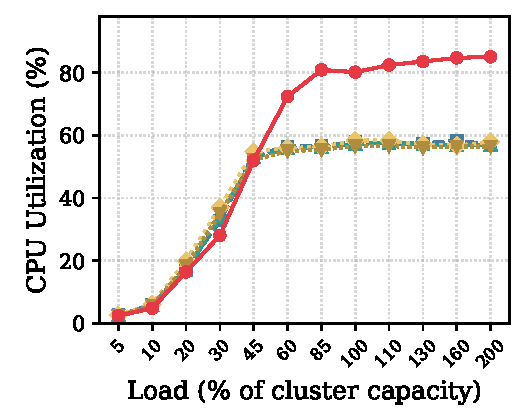
\includegraphics[width=0.31\linewidth]{figures/fig_main_cpu.pdf}\hfill
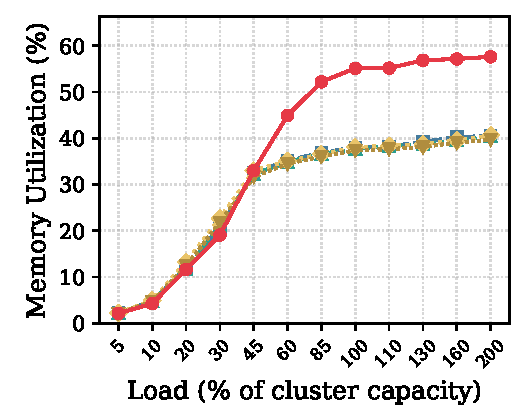
\includegraphics[width=0.31\linewidth]{figures/fig_main_mem.pdf}\hfill
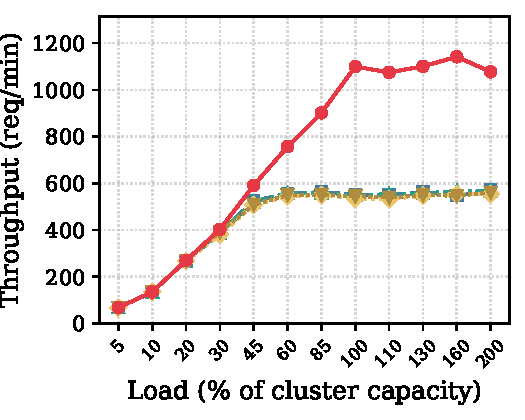
\includegraphics[width=0.31\linewidth]{figures/fig_main_throughput.pdf}\par
\small\textbf{Revised Figure 7: Main-experiment comparison across offered loads: (a) CPU utilization, (b) memory utilization, and (c) task throughput.}
\end{center}

\evidencefigure[0.50\linewidth]{figures/fig_main_latency.pdf}{Revised Figure 8: 99th-percentile latency across offered loads.}

\begin{revisionquote}
``Figures~7 and~8 compare COSMOS with the baselines across offered loads from 5\% to 200\% of cluster capacity. Unless otherwise stated, all reported differences are relative to the best-performing baseline for the corresponding metric at each load. At light loads (5\%--30\%), all systems achieve nearly identical throughput, with differences within 5.82\%, because resources are abundant and scheduling efficiency is not yet a bottleneck. The baselines also perform similarly, except that Golgi generally incurs higher tail latency, suggesting that its relatively aggressive overcommitment involves a tail-latency trade-off.

The advantage of COSMOS emerges as the offered load approaches cluster capacity. At 45\% load, COSMOS improves throughput by 12.83\% and reduces the 99th-percentile latency by 78.77\%. From 60\% to 200\% load, all baselines reach a similar throughput ceiling. In contrast, COSMOS improves CPU utilization by 28.34\%--46.91\%, memory utilization by 27.76\%--45.00\%, and throughput by 35.63\%--101.31\%. Over the same range, COSMOS reduces the 99th-percentile latency by 8.19\%--28.94\%, showing that its throughput gains do not compromise tail latency.

These gains stem from two complementary mechanisms. Complementary swarming narrows each node's function set to improve reuse while matching resource profiles to node capacity to reduce fragmentation. Monotonic scale-up further reduces over-provisioning and cold starts, sustaining higher utilization and throughput as load rises.''
\end{revisionquote}

Further, we provide a performance breakdown through simplified variants to quantify the contribution of each COSMOS component:

\begin{revisionquote}
``Figure~16 shows the performance comparison between COSMOS and simplified variants. We also provide the evaluation results of the baselines for reference.

As shown, Routing* performs between the baselines and COSMOS. At 100\% offered load, it improves CPU utilization, memory utilization, and task throughput over the best-performing baseline by 14.71\%, 16.80\%, and 28.57\%, respectively. However, it remains below COSMOS by 16.48\%, 19.36\%, and 35.57\% on the same metrics. These results show that complementary swarming alone improves resource efficiency and throughput, but requires monotonic scale-up for fine-grained intra-node resource management.

Scheduling* exhibits a different trade-off. Its CPU and memory utilization are 26.23\% and 12.19\% lower than COSMOS, respectively, while its throughput is 6.21\% higher. This result suggests that, without complementary routing, the node-local scheduler favors immediately schedulable requests and thereby increases the completed-request count, but does not align each node's workload with its multidimensional resource capacity. In contrast, COSMOS uses complementary routing to admit a more resource-efficient workload mix, substantially improving CPU and memory utilization at the cost of slightly lower throughput in this setting.''
\end{revisionquote}

\evidencefigure{figures/fig_ablation.pdf}{Revised Figure 16: Performance comparison among COSMOS, the baselines, and simplified variants.}

\begin{reviewcomment}
\textbf{Comment 2.3:} More comprehensive evaluations would strengthen the effectiveness of COSMOS. COSMOS relies on periodically generated routing plans, and this paper reports that plan generation is fast. It also uses steady-rate invocations in the experiments to avoid interference from burstiness. This makes me concerns about the effectiveness of COSMOS when the workload is rapidly shifting or difficult to predict? In realistic serverless environments, function popularity and request characteristics may change quickly, in which case a periodically generated routing plan may become stale. So, it would be better to explain and test more dynamic scenarios to demonstrate that COSMOS remains effective beyond relatively stable conditions.
\end{reviewcomment}
\response{2.3} Thank you for your suggestion. We revised and extended the experimental section to address the above concerns. We describe these changes below.

First, regarding the workload trace used in our experiments, we regenerated the scalability experiment using traces from the open-source Azure Functions Dataset and verified that the scheduler overhead remains within tens of milliseconds under real traces. In the revised manuscript, all request invocation traces are derived from the Azure dataset, which contains substantial real-world load changes and bursty fluctuations. The following revised text describes the workload characteristics and the scheduler-overhead results in the experimental section:

\begin{revisionquote}
``We generate user traffic based on the Azure Functions Dataset~[15]. For each benchmark, we randomly sample an invocation trace from the top 20\% most frequently invoked functions, which account for most production resource consumption~[15]. Their invocation-rate CV averages 55.36\% (range: 28.52--97.23\%), providing substantial temporal variation.''
\end{revisionquote}

\begin{quote}\small
[15] M.~Shahrad, R.~Fonseca, I.~Goiri, G.~Chaudhry, P.~Batum, J.~Cooke, E.~Laureano, C.~Tresness, M.~Russinovich, and R.~Bianchini, ``Serverless in the wild: Characterizing and optimizing the serverless workload at a large cloud provider,'' in \emph{Proceedings of the 2020 USENIX Annual Technical Conference}, California, USA, 2020, pp. 205--218.
\end{quote}

\begin{revisionquote}
``Between minutes 26 and 28, the invocation rate of \textbf{graph-pagerank} rises by about $5\times$. This burst is particularly challenging because \textbf{graph-pagerank} is among the most resource-demanding benchmarks.''
\end{revisionquote}

\evidencefigure[0.52\linewidth]{figures/fig_overhead_combined.pdf}{Revised Figure 18: Routing-plan generation and task-scheduling overhead under different cluster sizes and application workloads.}

\begin{revisionquote}
``We evaluate the overhead of the COSMOS scheduler under varying cluster sizes and user traffic. To do so, we simulate scheduler load for clusters ranging from 32 to 1024 worker nodes, scaling function load proportionally with cluster size and sweeping each cluster up to 150\% offered load. The experimental results are presented in Figure~18.

The upper panel of Figure~18 shows the average duration for COSMOS to generate cluster-wide request routing plans. It can be observed that the generation duration increases gradually with cluster scale but remains largely unaffected by invocation frequency. This is because COSMOS scales the overall load proportionally to the cluster size before computing the routing plan. Even with 1024 worker nodes and an invocation rate above $260 \times 10^3$ requests per minute, the latency stays below 60 ms. This result indicates that the scheduler can generate routing plans promptly, even in large-scale clusters, demonstrating the practical scalability of COSMOS.

The lower panel of Figure~18 shows the scheduling overhead for individual tasks under different scenarios. It should be noted that routing plan generation is performed by a separate background process within the scheduler. The main scheduling process only receives the resulting routing plan and assigns tasks accordingly. Therefore, only the scheduling overhead contributes to the additional latency in the end-to-end task execution path. As shown, even with 1024 worker nodes under heavy load, the extra scheduling delay added by COSMOS remains below 2.5 ms. This overhead is negligible for the vast majority of FaaS scenarios, confirming that the scheduling logic of COSMOS remains computationally lightweight at large cluster scales.''
\end{revisionquote}

Second, to more clearly investigate how COSMOS behaves when a sudden load shift makes a periodically generated routing plan stale, we set the routing-plan update interval to five minutes and evaluate how the system handles the bursty episode:

\evidencefigure[0.52\linewidth]{figures/fig_temporal_coldstart_latency.pdf}{Revised Figure 11: Minute-level cold-start rate and 99th-percentile tail latency under bursty load and routing-plan updates.}

\begin{revisionquote}
``Figure~11 shows the minute-level cold-start rate and 99th-percentile tail latency after excluding the first five minutes of system warm-up. We present results at 45\% offered load because the baselines already exhibit substantial request backlogs at 100\% load.

Between minutes 26 and 28, the invocation rate of \textbf{graph-pagerank} rises by about $5\times$. This burst is particularly challenging because \textbf{graph-pagerank} is among the most resource-demanding benchmarks. As shown in the figure, the burst causes sharp increases in both cold starts and tail latency for all systems. Nevertheless, COSMOS incurs fewer cold starts and a smaller latency spike than the baselines, and its tail latency quickly returns toward its pre-burst level. In contrast, the baselines retain elevated tail latency and recover more slowly.

This difference arises because complementary swarming confines individual function demand fluctuations to a small subset of servers, while the resulting resource-complementary load mix mitigates intra-server resource contention. Together, these properties limit both the cluster-wide impact of a burst and its performance interference with other functions. The baselines lack this isolation, allowing burst-induced contention and request backlogs to affect more servers and prolong latency recovery. For sustained workload changes, COSMOS revises the cluster load partition at the next routing-plan update to realign resources with demand.''
\end{revisionquote}

We also clarified the configurability of the routing-plan update period in the implementation section:

\begin{revisionquote}
``The routing plan generator runs as a periodic cluster-level service. It executes the complementary swarming routing algorithm to compute the optimized request routing plan, with an execution period of five minutes. This interval is configurable: it can be shortened for more volatile workloads or lengthened for stable workloads to reduce the performance disruption caused by load repartitioning.''
\end{revisionquote}

\begin{reviewcomment}
\textbf{Comment 2.4:} Since the related work section discusses many relevant systems, it would strengthen the evaluation to include comparisons against more state-of-the-art baselines, such as Golgi.
\end{reviewcomment}
\response{2.4} Thank you for your suggestion. We added Golgi as a new baseline in Section~VI. The experimental results show that COSMOS consistently maintains a performance advantage over Golgi:

\begin{revisionquote}
``Golgi~[43]: Golgi monitors instance performance using low-level runtime metrics and employs Mondrian Forest models to route requests between overcommitted and non-overcommitted instances. Since COSMOS does not support intra-instance task concurrency, we evaluate two implementations: Golgi, which approximates concurrency control in Golgi by adjusting instance resource allocations, and Golgi-NoCC, which omits this mechanism. The original Golgi study reports that disabling concurrency control changes performance by at most 14\%~[43], suggesting that performance monitoring and Mondrian Forest-based routing account for most of the system advantages. \ldots{} To ensure a fair comparison and minimize engineering artifacts, we reimplement all three baselines in our prototype following their respective papers. Other components of the prototype system are kept identical across all evaluated systems.''
\end{revisionquote}

\begin{revisionquote}
``Figures~7 and~8 compare COSMOS with the baselines across offered loads from 5\% to 200\% of cluster capacity. Unless otherwise stated, all reported differences are relative to the best-performing baseline for the corresponding metric at each load. At light loads (5\%--30\%), all systems achieve nearly identical throughput, with differences within 5.82\%, because resources are abundant and scheduling efficiency is not yet a bottleneck. The baselines also perform similarly, except that Golgi generally incurs higher tail latency, suggesting that its relatively aggressive overcommitment involves a tail-latency trade-off.

The advantage of COSMOS emerges as the offered load approaches cluster capacity. At 45\% load, COSMOS improves throughput by 12.83\% and reduces the 99th-percentile latency by 78.77\%. From 60\% to 200\% load, all baselines reach a similar throughput ceiling. In contrast, COSMOS improves CPU utilization by 28.34\%--46.91\%, memory utilization by 27.76\%--45.00\%, and throughput by 35.63\%--101.31\%. Over the same range, COSMOS reduces the 99th-percentile latency by 8.19\%--28.94\%, showing that its throughput gains do not compromise tail latency.

These gains stem from two complementary mechanisms. Complementary swarming narrows each node's function set to improve reuse while matching resource profiles to node capacity to reduce fragmentation. Monotonic scale-up further reduces over-provisioning and cold starts, sustaining higher utilization and throughput as load rises.''
\end{revisionquote}

\begin{center}

\includegraphics[width=0.60\linewidth]{figures/fig_main_legend.pdf}\\[-6pt]
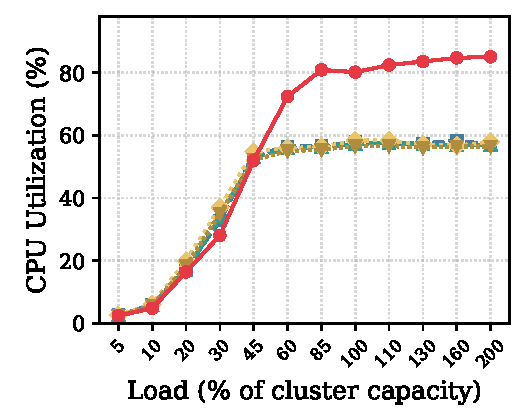
\includegraphics[width=0.31\linewidth]{figures/fig_main_cpu.pdf}\hfill
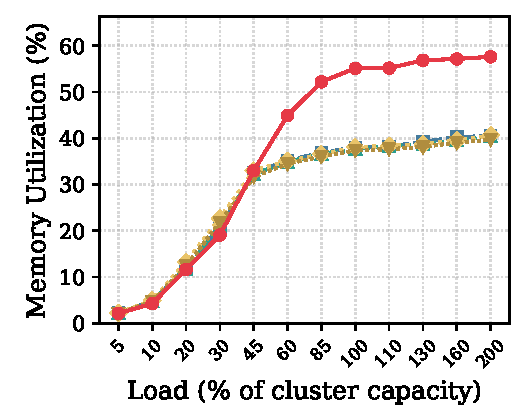
\includegraphics[width=0.31\linewidth]{figures/fig_main_mem.pdf}\hfill
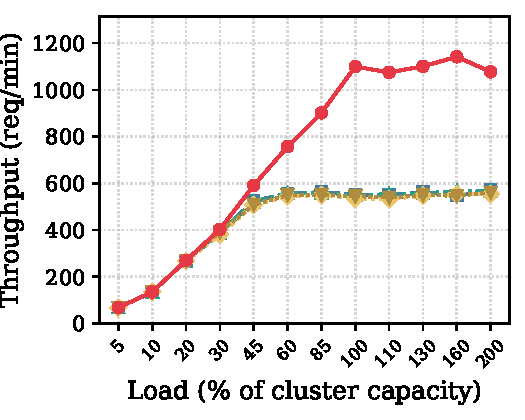
\includegraphics[width=0.31\linewidth]{figures/fig_main_throughput.pdf}\par
\small\textbf{Revised Figure 7: Main-experiment comparison across offered loads: (a) CPU utilization, (b) memory utilization, and (c) task throughput.}
\end{center}

\evidencefigure[0.50\linewidth]{figures/fig_main_latency.pdf}{Revised Figure 8: 99th-percentile latency across offered loads.}

We also added Golgi comparison results to the fine-grained performance analysis, generality experiments, and larger-scale cluster tests. For space reasons, we do not reproduce all of these results in the response letter; they are included in the revised manuscript.

\section*{Detailed Response to Reviewer 3}

\begin{reviewcomment}
\textbf{Comment 3.1:} I hope the authors could explicitly characterize the regime in which vertical scaling is fundamentally needed/ worth the extra management complexity. If requests are highly predictable and cleanly splittable/mergeable into a small number of size classes, then predictive horizontal scaling with prewarmed size-specific pools may recover most of the benefit without in-place vertical resizing? In that case, is vertical scaling still essential? The paper needs to explain why that regime is insufficient or too costly in practice.
\end{reviewcomment}
\response{3.1} Thank you for your comment. We agree that predictive horizontal scaling with size-specific prewarmed pools can recover much of the request-level allocation benefit when a function has only a few stable request types and the load of each type is highly predictable. However, this approach has an inherent granularity trade-off. If the pools are divided coarsely, a static size cannot closely match the resource demand of every request in the class, so within-class over-provisioning remains. If the pools are divided finely, the available prewarmed capacity is fragmented across many small pools; a burst in one size class can exhaust its corresponding pool and cause queuing or cold starts even when capacity in other pools remains idle. Monotonic scaling avoids this trade-off by allowing warm instances of the same function to serve requests of different sizes and adjust their allocations without predefined class boundaries. We added the following discussion in Section~VII:

\begin{revisionquote}
``A natural question is why predictive horizontal scaling with size-specific prewarmed pools cannot replace monotonic vertical scaling. Such pools face an inherent granularity trade-off. Coarse classes use static sizes that cannot closely match every request, retaining within-class over-provisioning. Fine classes fragment prewarmed capacity into many small pools; a burst in one class can cause queuing or cold starts even while warm instances in other classes remain idle. Monotonic vertical scaling avoids this trade-off by sharing warm instances across request sizes without predefined class boundaries. Size-specific pools remain effective when a function has only a few stable request types with predictable per-class load; otherwise, vertical scaling better accommodates heterogeneous and bursty demands.''
\end{revisionquote}

\begin{reviewcomment}
\textbf{Comment 3.2:} I hope the authors could better justify several core assumptions underlying the design. In particular, COSMOS relies on a per-function demand profile $\langle r_i,V_i,D_i\rangle$, where $r_i$ is assumed to be a fixed CPU-to-memory ratio across all requests of the same function, and requests are routed based on their position in the historical demand distribution $D_i$. This is a strong assumption that is currently asserted rather than validated. I believe it may hold when request demands vary mostly in scale, but it is less convincing for functions whose inputs induce qualitatively different CPU/memory behavior across requests. Since both the complementary routing policy and the monotonic queue ordering depend on this structure, the paper should clarify when this assumption is expected to hold and how sensitive the design is when it does not.

Also, the evaluation seems to assume accurate demand knowledge: it obtains ``accurate demand estimates'' from benchmark input characteristics, but does not justify how such estimates would be available in realistic deployments, or evaluate what happens when demand prediction is noisy, stale, or wrong. In addition, the evaluation assumes that CPU demand scales proportionally with a fixed CPU-to-memory ratio for each benchmark. I think the paper would be much stronger if it either justified why these assumptions are realistic for its target workloads, or included a robustness study showing how performance changes under imperfect demand estimation and non-constant per-request resource ratios.
\end{reviewcomment}
\response{3.2} Thank you for your comment. This comment raises two related but distinct questions: whether the fixed CPU-to-memory ratio is valid for the target workloads, and whether COSMOS relies on unrealistically accurate demand knowledge. We address them in this order.

First, we agree that the fixed-ratio assumption should be empirically justified rather than simply asserted. The assumption is motivated by a characteristic of serverless computing: complex, stateful applications are commonly decomposed into fine-grained, dedicated, stateless functions. Because each function performs a well-defined task, request inputs often change the magnitude of its demand without qualitatively changing its resource-use pattern. We added an empirical characterization in Section~II-B:

\begin{revisionquote}
``Figure~2 further examines how CPU and memory usage co-vary as request inputs change. We randomly select ten functions from the open-source SeBS serverless benchmarking suite~[37], covering Web, multimedia, utility, machine-learning, and scientific workloads; their full names and characteristics are listed in Table~I. For each input, we measure the CPU time consumed and peak memory usage during task execution, averaged across repeated runs. Each point represents one input, and the red line is a per-function linear fit. The reported $R^2$ measures the goodness of fit, while CV is the coefficient of variation of the per-input CPU-to-peak-memory ratios. The figure omits graph-mst due to space because it closely matches graph-bfs ($R^2=0.996$, CV=27.9\%).

Eight of the ten benchmarks exhibit strong input-dependent CPU--memory coupling: their CPU and memory demands increase along a stable function-specific direction, with linear-fit $R^2$ values between 0.974 and 0.999 and ratio CVs from 5.2\% to 29.7\%. Thus, although inputs change demand magnitude, the relative CPU-to-peak-memory profile remains broadly stable and does not typically switch between compute- and memory-intensive behavior. This property follows naturally from the fine-grained, single-purpose design of serverless functions: each invocation performs a well-defined task, while complex applications are commonly decomposed into multiple such functions. The remaining two benchmarks, video-processing and uploader, exhibit a streaming pattern: peak memory remains nearly constant while CPU consumption grows with input size.''
\end{revisionquote}

\evidencefigure{figures/fig_ratio_stability_grid.pdf}{Revised Figure 2: CPU and memory usage across request inputs for serverless functions.}

Based on this evidence, we also clarified the scope and boundary cases of the fixed-ratio model in the Discussion. Single-resource-dominant functions can be represented conservatively, whereas complex functions whose resource profiles change qualitatively across requests are not directly supported:

\begin{revisionquote}
``Serverless computing commonly decomposes complex, stateful applications into fine-grained, dedicated, stateless functions that scale independently, with state externalized to storage services. Because each function performs a well-defined task, request inputs often change demand magnitude rather than its qualitative CPU-to-memory profile, as illustrated by eight of the ten functions in Figure~2. Motivated by this structure, COSMOS models each function with a stable CPU-to-memory demand ratio and a variable demand magnitude.

Single-resource-dominant functions, such as video-processing and uploader in Figure~2, can still be represented by a conservative fixed resource ratio. This may over-allocate the less-variable resource but preserves normal system operation. Specialized support would require extending the demand model and SwapCapacity routine to allow the ratio to vary with request size.

The current model does not directly support a complex function whose resource profile changes qualitatively across requests. Such a function could be divided into virtual functions by request type or refactored into dedicated stages, each with a stable profile. We leave direct support for such functions to future work.''
\end{revisionquote}

Second, regarding demand knowledge, we clarify that the phrase ``accurate demand estimates'' in the initial submission was an overstatement, and we have revised the corresponding wording. For the target workloads described above, obtaining a useful request-level estimate is generally straightforward: we profile historical executions and fit first- to second-order functions from request scale to CPU and peak-memory demand. The stable profiles in Figure~2 explain why this simple procedure is sufficient for most evaluated functions.

COSMOS does not assume access to an oracle estimator, nor does its performance advantage come from a predictor that is more accurate than those used by the baselines. All evaluated systems use the same request-level resource-demand estimation method, except Golgi, which retains its own overcommitment mechanism. COSMOS differs in how it uses the resulting estimates for request routing and task scheduling. We clarified these algorithm inputs and the prototype estimation procedure in the Discussion:

\begin{revisionquote}
``As shown in Section~IV-B, COSMOS requires cluster node capacities and function resource-demand information when constructing routing and scheduling decisions. Node capacities are normally available to the scheduler, whereas function resource-demand modeling requires measurements from historical executions. COSMOS also consumes predictions of future per-function load and request-level resource demand. These predictions can be supplied by any demand forecasting algorithm, but the algorithms themselves fall outside the scope of this paper. In the prototype system, we use an FFT-based prediction algorithm to forecast future load and employ first- to second-order linear fitting functions of request scale to predict per-request resource demands. These simple strategies have proven sufficient to meet the system requirements. Furthermore, COSMOS exhibits a certain tolerance towards inaccuracies in future load prediction, as shown in Figure~15.''
\end{revisionquote}

Finally, we distinguish request-level demand estimation from future per-function load prediction. The former is shared by the evaluated systems, whereas COSMOS uniquely uses the latter to generate routing plans. We therefore additionally evaluate COSMOS under different levels of future-load prediction error. The results show that its advantage over the baselines does not rely on exact future-load prediction:

\begin{revisionquote}
``Figure~15 compares COSMOS without injected prediction errors against variants with $\pm$10\% and $\pm$20\% random errors and $\pm$15\% systematic biases across offered loads. For a $\pm x\%$ random-error setting, we independently multiply each function's predicted load at every routing update by $1+\epsilon$, where $\epsilon$ is uniformly sampled from $[-x,x]$. For a $\pm y\%$ systematic-bias setting, every predicted function load is multiplied by the fixed factor $1+y$ or $1-y$, respectively. For readability, we show only Palette and FaaSCache as representative baselines. When offered load remains within cluster capacity, the impact of injected errors remains bounded because available resource slack can absorb moderate allocation inaccuracies: relative to the unperturbed setting, throughput deviates by at most 9.79\%, while CPU and memory utilization deviate by at most 13.70\% and 7.61\%, respectively. Once load exceeds cluster capacity, inaccurate predictions can create imbalanced allocations, producing less stable performance across load levels; independently sampled errors further amplify this variability across functions and routing-plan updates. Nevertheless, all prediction-error variants retain a clear and consistent advantage over the baselines, indicating that COSMOS's overall performance gains are robust to imperfect demand estimates.''
\end{revisionquote}

\begin{center}

\includegraphics[width=0.84\linewidth]{figures/fig_robustness_legend.pdf}\\[-6pt]
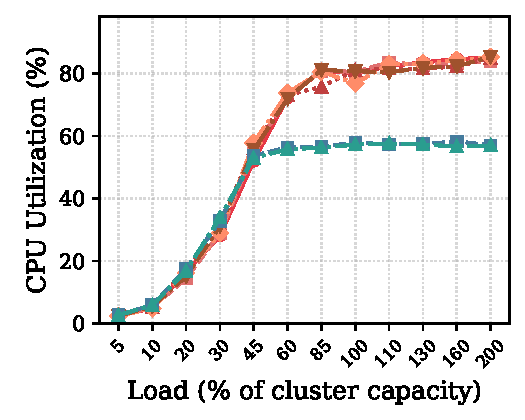
\includegraphics[width=0.31\linewidth]{figures/fig_robustness_cpu.pdf}\hfill
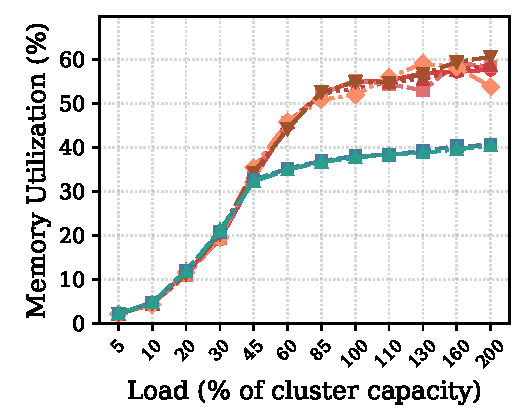
\includegraphics[width=0.31\linewidth]{figures/fig_robustness_mem.pdf}\hfill
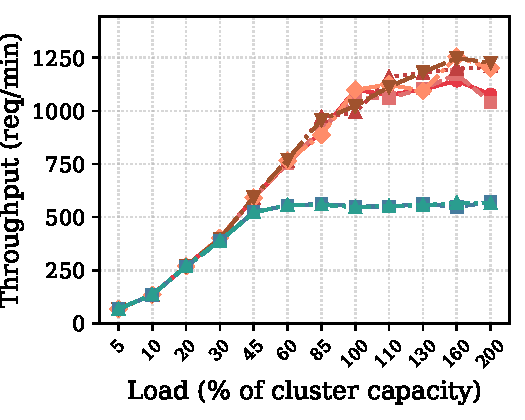
\includegraphics[width=0.31\linewidth]{figures/fig_robustness_throughput.pdf}\par
\small\textbf{Revised Figure 15: Robustness under demand-prediction errors.}
\end{center}

\begin{reviewcomment}
\textbf{Comment 3.3:} The scale-up scheduling avoids downscaling at the function level, but at a node level eviction may have to be triggered frequently if no downscaling is performed. It is not clear how much the proposed policy actually resolves the dynamic resource allocation problem, rather than shifting intra-function scaling overhead into inter-function contention and eviction pressure. I think the paper should better clarify this distinction and quantify how often scale-up can be absorbed by slack versus causing eviction or delayed execution.
\end{reviewcomment}
\response{3.3} Thank you for your suggestion. Under COSMOS's algorithmic mechanism, the total resource footprint of a function is not monotonically increasing; instead, it depends jointly on the number of active instances and their resource allocation. Resource contention can trigger instance eviction, thereby changing the number of available instances for a function. Even when the instance count remains stable, larger instances with higher resource allocations are more likely to be evicted, while newly created instances are typically smaller. To further clarify the impact of COSMOS's scale-up mechanism, we added the scale-up absorption breakdown, pod-eviction frequency, and function instance-lifetime analysis in Section~VI-C.

First, Figure~13 quantifies how often requested scale-up is absorbed by available node resources rather than causing pod eviction:

\begin{revisionquote}
``Figure~13 reports the fraction of scale-up events that trigger pod eviction across offered loads, \ldots{} Together with the overall pod-eviction rate and cold-start results, these metrics evaluate whether the eviction-amplification risk of in-place scaling translates into increased instance~churn.

For COSMOS, the fraction of scale-ups causing eviction first increases and then decreases with load. At light loads, eviction events initially grow faster than scale-up events. As load increases further, however, scale-ups become much more frequent and are predominantly absorbed by available node resources. From 45\% to 100\% load, the number of scale-up events increases by $6.34\times$, whereas the number causing eviction increases by only $1.48\times$; consequently, their fraction falls from 5.05\% to 1.18\%. Across COSMOS and all baselines, fewer than 15\% of scale-up events cause an eviction, indicating that in-place scale-up usually preserves warm instances rather than triggering additional cold starts.''
\end{revisionquote}

\evidencefigure[0.47\linewidth]{figures/fig_scaleup_absorption.pdf}{Revised Figure 13: Fraction of scale-up events that cause pod eviction.}

Second, we provide a comparison of instance eviction behavior between COSMOS and the baseline~systems:

\begin{revisionquote}
``Table~II reports the observed runtime pod eviction rates. \ldots{} Moreover, COSMOS incurs fewer cold starts than the baselines, and its pod-eviction rate is 1.433 events/min, 60.6\% lower than the best baseline in Table~II. These results show that routing-plan relocation does not increase observable instance churn.''
\end{revisionquote}

\begin{center}
\small
\begin{tabular}{lccccc}
\toprule
\textbf{System} & \textbf{Palette} & \textbf{FaaSCache} & \textbf{Golgi} & \textbf{Golgi-NoCC} & \textbf{COSMOS} \\
\midrule
Average rate (events/min) & 5.433 & 4.500 & 8.967 & 3.633 & \textbf{1.433} \\
\bottomrule
\end{tabular}\par
\vspace{2pt}\small\textbf{Revised Table II: Pod eviction rate among COSMOS and baselines for Figure~11.}
\end{center}

These results indicate that the scale-up mechanism does not introduce additional eviction pressure. Instead, by avoiding frequent cold starts and bidirectional resource-adjustment overhead, COSMOS improves resource-utilization efficiency and reduces resource contention, thereby reducing eviction pressure.

\evidencefigure{figures/fig_instance_lifetime_cdf.pdf}{Revised Figure 14: Instance-lifetime distributions.}

Finally, we report the function instance-lifetime statistics. COSMOS produces longer instance lifetimes across different functions, indicating that COSMOS improves instance reuse across different functions rather than increasing inter-function contention:

\begin{revisionquote}
``Figure~14 compares the instance-lifetime distributions of four representative functions. \ldots{} Consistent with this result, the instance-lifetime CDFs in Figure~14 shift toward longer lifetimes under COSMOS. We observe the same trend for the remaining six functions. These results show that monotonic scale-up does not increase instance churn.''
\end{revisionquote}

\vspace{12pt}
% The third part of the final response package will append the complete revised
% manuscript with all modifications highlighted in blue. It is intentionally
% omitted from this draft.

\end{document}
